\documentclass{article}
\usepackage{algorithm}
\usepackage{algpseudocode}
\usepackage{amsmath,amssymb,amsthm}
\usepackage{graphicx}
\usepackage[margin=1in]{geometry}
\usepackage{fancyhdr}
\usepackage{float}
\usepackage{longtable}
\newcommand{\bx}{{\bf x}}
\newcommand{\bw}{{\bf w}}
\newcommand{\bb}{{\bf b}}
\newcommand{\bv}{{\bf v}}
\newcommand{\by}{{\bf y}}
\setlength{\parindent}{0pt}
\setlength{\parskip}{5pt plus 1pt}
\setlength{\headheight}{13.6pt}
\newcommand\question[2]{\vspace{.25in}\hrule\textbf{#1: #2}\hrule\vspace{.10in}}
\renewcommand\part[1]{\vspace{.10in}\textbf{(#1)}}
\newcommand\algo{\vspace{.10in}\textbf{Algorithm: }}
\newcommand\correctness{\vspace{.10in}\textbf{Correctness: }}
\newcommand\runtime{\vspace{.10in}\textbf{Running time: }}
\newcommand\pseudoCode{\vspace{.10in}\textbf{PseudoCode: }}
\newcommand*{\perm}[2]{{}^{#1}\!P_{#2}}
\newcommand*{\comb}[2]{{}^{#1}\!C_{#2}}
%\pagestyle{fancyplain}
%\lhead{\textbf{\NAME\ (\UID)}}
%\chead{\textbf{Hw\HWNUM}}
%\rhead{CS 6350, \today}
\title{CS6210 - Homework/Assignment-5}
\author{Arnab Das(u1014840)}
\usepackage[utf8]{inputenc}
\begin{document}
  \pagenumbering{gobble}
  \maketitle
  \newpage
  \pagenumbering{arabic}
  \newcommand\NAME{ARNAB DAS}
  \newcommand\UID{uxxxxxxx}
  \newcommand\HWNUM{4}



\question{1}{Chapter-9: Question-5}
An $n \times n$ linear system of equations $Ax=b$ is modified such that every $b_i$ is replaced with $b_i - x_i^3$. \newline\part{a} For the system $Ax=b$, thus we have: \newline
A = $\begin{bmatrix}
	a_{11} & a_{12} & a_{13} & \dots & a_{1n} \\
	a_{21} & a_{22} & a_{23} & \dots & a_{2n} \\
	\dots & \dots & \dots & \dots & \dots \\
	a_{n1} & a_{n2} & a_{n3} & \dots & a_{nn} \\
\end{bmatrix}$ , $x$ = $\begin{bmatrix}
			x_1 \\
			x_2 \\
			\dots \\
			x_n \\
\end{bmatrix}$ and $b$ = $\begin{bmatrix}
			b_1 \\
			b_2 \\
			\dots \\
			b_n \\
			\end{bmatrix}$ \newline
The b vector gets modified as $\begin{bmatrix} 
				b_1 - x_1^3 \\
				b_2 - x_2^3 \\
				\dots \\
				b_n - x_n^3 \\
\end{bmatrix}$, so that now we have a non-linear system that can be expressed as \textbf {f(x)=}, where f is a vector of functions represented as :
\[ f_1(x) = (a_{11}x_1 + x_1^3) + a_{12}x_2 + \dots + a_{1n}x_n - b_1 = 0\]
\[ f_2(x) = a_{21}x_1 + (a_{22}x_2 + x_2^3) + \dots + a_{2n}x_n - b_2 = 0\]
\[ \dots \]
\[ f_i(x) = a_{i1}x_1 + a_{i2}x_2 + \dots + (a_{ii}x_i + x_i^3) + \dots + a_{in}x_n - b_i = 0\]
\[ \dots \]
\[ f_n(x) = a_{n1}x_1 + a_{n2}x_2 + \dots + a_{nn}x_n + x_n^3 - b_n = 0\]

Then, the Jacobian of this vector of functions, f, will be: \newline
J = $\begin{bmatrix}
	\dfrac{\partial f_1}{\partial x_1} & \dfrac{\partial f_1}{\partial x_2} & \dfrac{\partial f_1}{\partial x_3} & \dots & \dfrac{\partial f_1}{\partial x_n}\\
	\dfrac{\partial f_2}{\partial x_1} & \dfrac{\partial f_2}{\partial x_2} & \dfrac{\partial f_2}{\partial x_3} & \dots & \dfrac{\partial f_2}{\partial x_n}\\
	\dots & \dots & \dots & \dots & \dots \\
	\dfrac{\partial f_n}{\partial x_1} & \dfrac{\partial f_n}{\partial x_2} & \dfrac{\partial f_n}{\partial x_3} & \dots & \dfrac{\partial f_n}{\partial x_n}\\
\end{bmatrix}$\newline \newline = $\begin{bmatrix}
		(a_{11} + 3x_1^2) & a_{12} & a_{13} & \dots & a_{1i} & \dots & a_{1n} \\
		a_{21} & (a_{22} + 3x_2^2) & a_{23} & \dots & a_{2i} & \dots & a_{2n} \\
		\dots & \dots & \dots & \dots & \dots & \dots & \dots \\
		a_{i1} & a_{i2} & a_{i3} & \dots & (a_{ii} + 3x_i^2) & \dots & a_{in} \\
		\dots & \dots & \dots & \dots & \dots & \dots & \dots \\
		a_{n1} & a_{n2} & a_{n3} & \dots & a_{ii} & \dots & (a_{in} + 3x_n^2) \\
		 \end{bmatrix}$ = A + D, where D is: \newline \newline
		 D = $\begin{bmatrix}
			 3x_1^2 & 0 & 0 & \dots & 0 & \dots & 0 \\
			 0 & 3x_2^2 & 0 & \dots & 0 & \dots & 0 \\
			\dots & \dots & \dots & \dots & \dots & \dots & \dots \\
			 0 & 0 & 0 & \dots & 3x_i^2 & \dots & 0 \\
			\dots & \dots & \dots & \dots & \dots & \dots & \dots \\
			 0 & 0 & 0 & \dots & 0 & \dots & 3x_n^2 \\
		      \end{bmatrix}$ \newline

  \part{b} Given that A is strictly diagonally dominant with positive elements in its diagonal. We know that a  strictly diagonally dominant matrix is non-singular, hence \textbf {A is non-singular}. Now, diagonal dominance means:
  \[ \forall i, |a_{ii}| \geq \sum_{j=1}^n |a_{ij}|, j \neq i\]
  Since, D is a diagonal matrix with non-negative elements along its diagonal, hence adding D to A, conserves the diagonal dominance in the resulting matrix J. Thus, at any iterate, the Jacobian, J, also remains diagonally dominant and hence non-singular. \newline

  \part{c} In Newton's method, we are theoretically basically solving the following:
  \begin{equation}
	  x_{k+1} - x_k = -J(x_k)f(x_k)
	  \label{eq:newton}
  \end{equation}
  where, $x_k$ is the value of x in the k'th iteration. For convergence of the method, we want the following:
  \begin{equation}
	  \dfrac{|| x_{k+1} - x^*||}{||x_k - x^*||} = \lambda
	  \label{eq:conv}
  \end{equation}
  where, $\lambda$ is some positive constant, and $x^*$ is the optimal solution. \newline
  The error at the (k+1)'th iteration can be written as:
  \begin{equation}
	  ||e_{k+1}|| = || x_{k+1} - x^*|| = || x_k - J(x_k)^{-1}f(x_k) - x^*|| = || e_k - J(x_k)^{-1}f(x_k) ||
  \label{eq:cerr}
  \end{equation}

  Now, from Taylor's series expansion, we have:
  \[f(x_k) = f(x^*) + J(x_k)(x_k - x^*) + \dfrac{1}{2}(x_k - x^*)^TH(x_k)(x_k - x^*) + \dots\]
  Approximating higher order terms:
  \[f(x_k) = f(x^*) + J(x_k)e_k + \dfrac{1}{2}(e_k)^TH(x_k)(e_k) \]

  At the optima, $f(x^*)=0$. Multiplying both sides by $J(x_k)^{-1}$ thus we get:
  \[ J(x_k)^{-1} f(x_k) = 0 + e_k +  \dfrac{1}{2}J(x_k)^{-1}(e_k)^TH(x_k)(e_k)\]

  Replacing this in $\eqref{eq:cerr}$
  \begin{equation}
   ||e_{k+1}|| = || e_k - e_k - \dfrac{1}{2}J(x_k)^{-1}(e_k)^TH(x_k)(e_k) || = ||\dfrac{1}{2}J(x_k)^{-1}(e_k)^TH(x_k)(e_k) || \leq \dfrac{||J^{-1}|| ||H||}{2} ||e_k||^2
   \label{eq:finalConv}
  \end{equation}

  Thus $\eqref{eq:finalConv}$ indicates that if the Jacobian is non-singular, then it quadratically converges. So, the only remaining peice is to show that the Jacobian is non-singular. We know that a symmetric positive definite matrix is non-singular. If we can proove that J is symmetric positive definite, then it suites our purpose: Consider any non-zero vector, \textbf {u}, then:
  \[u^T J u = u^T (A + D) u = u^TAu + u^TDu\]
  we know that A is symmetric positive definite, hence $u^TAu > 0$. So, we need to show now $u^TDu > 0$. \newline
  $u^TDu$ = $\begin{bmatrix}
	       u_1 & u_2 & \dots & u_n \\
	    \end{bmatrix}$ $\begin{bmatrix}
		    		3x_1^2 & 0 & 0 & \dots & 0 \\
				0 & 3x_2^2 & 0 & \dots & 0 \\
				\dots & \dots & \dots & \dots & \dots \\
				0 & 0 & 0 & \dots & 3x_n^2 \\
			    \end{bmatrix}$ $\begin{bmatrix}
				    		u_1 \\
						u_2 \\
						\dots \\
						u_n \\
				    	   \end{bmatrix}$ = $x_1^2u_1^2 + x_2^2u_2^2 + \dots + x_i^2u_i^2 + \dots + x_n^2u_n^2 > 0$ \newline

  Hence,
  \[u^T J u = u^T (A + D) u = u^TAu + u^TDu > 0\]
  Thus, the Jacobian is also symmetric positive definite and hence invertible and non-singular. Hence, it is guaranteed to converge as per $\eqref{eq:finalConv}$. \newline


	  	  

 


\question{2}{Chapter-9: Question-6}

\part{a} Given a linear system of equations, $Ax=b$, on which we apply Newton's method. For a linear system, the Jacobian, J, will be :
J = $\begin{bmatrix}
	\dfrac{\partial f_1}{\partial x_1} & \dfrac{\partial f_1}{\partial x_2} & \dfrac{\partial f_1}{\partial x_3} & \dots & \dfrac{\partial f_1}{\partial x_n}\\
	\dfrac{\partial f_2}{\partial x_1} & \dfrac{\partial f_2}{\partial x_2} & \dfrac{\partial f_2}{\partial x_3} & \dots & \dfrac{\partial f_2}{\partial x_n}\\
	\dots & \dots & \dots & \dots & \dots \\
	\dfrac{\partial f_n}{\partial x_1} & \dfrac{\partial f_n}{\partial x_2} & \dfrac{\partial f_n}{\partial x_3} & \dots & \dfrac{\partial f_n}{\partial x_n}\\
\end{bmatrix}$\newline \newline = $\begin{bmatrix}
		a_{11} & a_{12} & a_{13} & \dots & a_{1i} & \dots & a_{1n} \\
		a_{21} & a_{22} & a_{23} & \dots & a_{2i} & \dots & a_{2n} \\
		\dots & \dots & \dots & \dots & \dots & \dots & \dots \\
		a_{i1} & a_{i2} & a_{i3} & \dots & a_{ii} & \dots & a_{in} \\
		\dots & \dots & \dots & \dots & \dots & \dots & \dots \\
		a_{n1} & a_{n2} & a_{n3} & \dots & a_{ii} & \dots & a_{in} \\
		 \end{bmatrix}$ = A  \newline

 Thus, Newton's method applied to this problem becomes:
 \[ x^* = x_1 = x_0 + A^{-1}(b - Ax_0) = A^{-1}b\]
 Hence, it will converge in a single iteration.

 \part{b}
 The Newton's method is of the form:
 \[ J(x_k)(x_{k+1} - x_k) = -f(x_k)\]

 If the Jacobian is singular at the solution, then theoretically it means $\Delta x_k = x_{k+1} - x_k$, will be potentially large in the region close to the solution which means the values of x at the k'th and (k+1)'th iterate will have a large difference implying that convergence will be extremely slow and even the convergence might be lost, since two consecutive iterations will not result in close 'x' values that can meet the convergence limits. Also, since J is singular, hence the condition numner given by $||J||||J^{-1}||$ will be infinitely large indicating an ill-conditioned system, which will not potentially converge. \newline




\question{5}{Chapter-10: Question-6}
Given 4 data points as below:
\[(x_0,y_0) = (-1,1)\]
\[(x_1,y_1) = (0,1)\]
\[(x_2,y_2) = (1,2)\]
\[(x_3,y_3) = (2,0)\]

\part{Monomial Basis} 
\[ p(x) = \sum_{j=0}^3 c_jx^j\]
where $c_j$ are the coefficients of the j'th basis. \newline

At $(x_0, y_0)$, 
\[p(x_0) = p(-1) = c_0 - c_1 + c_2 - c_3 = y_0 = 1\]

At $(x_1, y_1)$,
\[p(x_1) = p(0) = c_0 = y_1 = 1\]

At $(x_2, y_2)$,
\[ p(x_2) = p(1) = c_0 + c_1 + c_2 + c_3 = 2 \]

At $(x_3, y_3)$,
\[ p(x_3) = p(2) = c_0 + 2c_1 + 4c_2 + 8c_3 = 0\]

Combining these above 4 equations, we get the following system of equations: \newline
$\begin{bmatrix} 
	1 & -1 & 1 & -1 \\
	1 & 0 & 0 & 0 \\
	1 & 1 & 1 & 1 \\
	1 & 2 & 4 & 8 \\
\end{bmatrix}$ $\begin{bmatrix}
			c_0 \\
			c_1 \\
			c_2 \\
			c_3 \\
\end{bmatrix}$ = $\begin{bmatrix}
			1 \\
			1 \\
			2 \\
			0 \\
		  \end{bmatrix}$

Solving this system of equation, we get the following coefficients values for monomial basis: \newline
\hspace*{0.5cm} $c_0 = 1$, $c_1 = 1.16667$, $c_2 = 0.5$, $c_3 = -0.6667$ \newline
Thus the interpolating cubic polynomial using monomial basis will be:
\begin{equation}
	p(x) = 1 + 1.6667 x + 0.5x^2 - 0.6667 x^3
 \label{eq:mono}
\end{equation}

\part{Lagrange}

In the Lagrange, the j'th basis function is defined as:
\[ L_j(x) = \dfrac{(x-x_0) \dots (x - x_{j-1})(x - x_{j+1}) \dots (x - x_n)}{(x_j-x_0) \dots (x_j - x_{j-1})(x_j - x_{j+1}) \dots (x_j - x_n)}\]

and the polynomial is defined as: \newline
$p(x) = \sum_{j=0}^n y_j L_j(x) = 1\dfrac{(x-0)(x-1)(x-2)}{(-1-0)(-1-1)(-1-2)} + 1\dfrac{(x+1)(x-1)(x-2)}{(0+1)(0-1)(0-2)} + 2 \dfrac{(x+1)(x-0)(x-2)}{(1+1)(1-0)(1-2)} + 0.L_3(x) = \dfrac{-4x^3 + 3x^2 + 7x + 6}{6}$


Hence, we get the following coefficient values for the Lagrange's basis: \newline
\hspace*{0.5cm} $c_0 = 1$, $c_1 = 1.16667$, $c_2 = 0.5$, $c_3 = -0.6667$ \newline
Hence, the interpolating cubic polynomial with Lagrange basis will be , \newline
\begin{equation}
1 + 1.16667 x + 0.5 x^2 - 0.667x^3
	\label{eq:lagrange}
\end{equation}


\part{Newton} For a cubic interpolant, the basis functions will be: \newline
$\phi_0(x) = 1$, $\phi_1(x) = x - x_0 = x+1$ , $\phi_2(x) = (x-x_0)(x-x_1) = (x-x_0)x$, and $\phi_3(x) = (x-x_0)(x-x_1)(x-x_2) = (x+1)x(x-1) = (x^3 - x)$ \newline

	At $(x_0,y_0)$ \newline
	$p(-1)$ = $c_0$ = 1 \newline

	At $(x_1, y_1)$ \newline
	$p(0)$ = 1 + $c_1(x-x_0)$ = $y_1 => c_1 = 0$ \newline

	At $(x_2, y_2)$ \newline
	$p(1) = 1 + 0 + c_2(x-x_0)(x-x_1)$ = $y_2 => 1 + c_2(1+1)(1-0) = 2 => c_2 = \dfrac{1}{2}$  \newline

	At $(x_3, y_3)$ \newline
	$P(2) = 1 + 0 + c_2(2+1)(2-0) + c_3(2+1)(2-0)(2-1) = 0, => c_3 = \dfrac{-2}{3}$ \newline

	Hence, reconstructing the polynomial:
	\[p(x) = 1 + 0 + \dfrac{1}{2}x(1+x) - \dfrac{2}{3}(x+1)x(x-1)\]
	\[p(x) = 1 + \dfrac{7}{6}x + \dfrac{x^2}{2} - \dfrac{2}{3}x^3 \]
	\[p(x) = 1 + 1.1667 x + 0.5 x^2 - 0.667 x^3\]
Hence, the interpolating cubic polynomial with Lagrange basis will be , \newline
\begin{equation}
1 + 1.16667 x + 0.5 x^2 - 0.667x^3 
	\label{eq:nbasis}
\end{equation}

	As $\eqref{eq:mono}$, $\eqref{eq:lagrange}$ and $\eqref{eq:nbasis}$ shows that the three representations gives the same polynomial. \newline


\question{7}{Chapter-10: Question-25}

\part{a} Let the quadratic polynomial be 
\begin{equation}
	p(x) = c_0 + c_1 x + c_2 x^2
	\label{eq:quad}
\end{equation}

Then , at x=0:
\[ p(0) = c_0 = f(0) = 1 \]
and
\[ p^\prime(0) = c_1 = f^\prime(0) = -1\]

At, x=1:
\[ c_0 + c_1 + c_2 = f(1) = 2 \]
Solving the above 3 equations, gives
\[ c_0 = 1\]
\[ c_1 = -1\]
\[ c_2 = 2\]

Plugging these coefficients back to $\eqref{eq:quad}$, we get the following quadratic interpolant:
\begin{equation}
	p(x) = 1 - x + 2x^2
	\label{eq:poly}
\end{equation}

By taking the first derivative and the second derivative of $\eqref{eq:poly}$, we get:
\[p^\prime(x) = -1 + 4x\]
\[p^{\prime\prime}(x) = 4 > 0\]
Equating the first derivative to 0, we get a stationary point at $x=\dfrac{1}{4}$, and since the second derivative, $p^{\prime\prime}(x) > 0$, hence this point is a minima. Thus we have found  $x^* = \dfrac{1}{4}$. (Answer) \newline

\part{b}
We already found the minima $x^* = \dfrac{1}{4}$ which is $0 < \dfrac{1}{4} < 1$. Since, it is quadratic, it has only a single maxima or minima becuase its first derivative is linear and hence cannot have multiple roots. Since, we have found a minima, hence it has to be the unique minima satisfying $0 < x^* < 1$. 
For the original function, given it has continuous second order derivative, however nothing is mentioned about its higher derivatives. Now, since $f(1) > f(0)$, there is a point in $[0,1)$, from where the function f starts to increase. Since, $f^\prime(0) < 0$, hence $x=0$ is not the point where f achieves a minimum. So, f achieves a minimum at $x^* = 0 + \delta$, where $\delta$ is a positive quantity between 0 and 1. Hence, f has a unique minimum at a point $0 < x < 1$ .Since , f has continuous second order derivative in this region, we do not know about its higher order derivatives. If it is quadratic, then this minima is unique for same reasons as the quadratic polynomial. But , if the underlying function is not quadratic, then the uniqueness cannot be asserted since there can be many more minimas in this region. 


\question{8}{Chapter-11: Question-3}
Let $f \in C^3[a,b]$ be given at equidistant points, $x_i = a + ih,$ where $i=0,1,2, \dots, n$ and $nh = b-a$. $f^\prime(a)$ is given as well. \newline

\part{a} Construct an algorithm for $C^1$ continuous quadratic interpolation: \newline
\[ v(x) = S_i(x) = a_i + b_i(x - x_i) + c_i(x - x_i)^2 ; x_i \leq x \leq x_{i+1}\]
That is an algorithm to determine the 3n coefficients. \newline

\algo
 The polynomial $S_i(x)$ in the interval $x_i \leq x \leq x_{i+1}$ will match the function value exactly. So, we have our first condition as:
	\[S_i(x_i) = a_i = f(x_i) \]
Thus, we have n equations in n variables due to this.
This gives us all the n $a_i$ values. \newline

Also, since $S_i(x)$ is valid in the interval $x_i \leq x \leq x_{i+1}$, hence it should satisfy the function value at $x_{i+1}$ as well. Thus we have our next condition as: 
\[ S_i(x_{i+1}) = f(x_{i+1}) \]
\[ a_i + b_i(x_{i+1} - x_i) + c_i(x_{i+1} - x_i)^2 = f(x_{i+1})\]
since, $x_{i+1} - x_i = h$, we get:
\[ b_i h + c_i h^2 = a_{i+1} - a_i\]
This gives us n equations in 2n variables. In combination with the above we get 2n equations in 3n variables. \newline

Next, since we want the interpolant to be $C^1$ continuous and the given fucntion is $C^3$, hence, the first derivative of $S_i(x_i)$ should match the first derivative of the function at $x_i$. Thus, we get: 
\[ S_{i}^\prime(x_i) = f^\prime(x_i) \]
\[ b_i = f^\prime(x_i)\]

Also, the derivatives should match at $x_{i+1}$. Hence, 
\[ S_i^\prime(x_{i+1}) = f^\prime(x_{i+1})\]
\[ b_i + 2c_i(x_{i+1} - x_i) = f^\prime(x_{i+1})\]
\[ b_i + 2c_i h = f^\prime(x_{i+1})\]

There is a certain pattern that emerges. If we know the derivative value at $x_i$, we can use it further to compute the derivative value at $x_{i+1}$. Since, we need to evaluate all the derivative values exceopt the first one, let us denote the derivative with the variable $d_i$. \newline
Thus, from the above relations we have the following set of equations:

n equations for
\[ a_i = f(x_i)\]

n equations for
\[ b_i h + ci h^2 - (a_{i+1} - a_i) = 0\]

n equations for 
\[ b_i - d_i = 0\]

(n-1) equations for 
\[ b_i + 2c_i h - d_{i+1} = 0 \]

1 equations for the derivative given at x=a, that is $d_0$
\[ d_0 = f(a)\]

Thus, in total we have 4n variables with 4n equations which can be solved to get the 3n coefficients $\{a_i, b_i, c_i\}$ and the derivatives $d_i$. \newline

\textbf{One more method:} Since, we want the piecewise interpolant to be $C^1$ continuous, hence at the interior point $x_i$, the first derivative of $S_{i-1}(x)$ should equal the first derivative of $S_i(x)$. Hence, we have the following relation:
\[ S_{i-1}(x_i) = S_i(x_i)\]
\[ b_{i-1} + 2c_{i-1}(x_i - x_{i-1}) = b_i\]
\[ b_{i-1} - b_i + 2c_{i-1} h = 0\]
This will have (n-1) equations since we equate between two consecutive interior points. \newline
Thus, now we can consider the following set of equations: \newline
n equations for
\[ a_i = f(x_i)\]

n equations for
\[ b_i h + ci h^2 - (a_{i+1} - a_i) = 0\]

(n-1) equations for 
\[ b_{i-1} - b_i + 2c_{i-1} h = 0\]

and 1 equation for the condition that the derivative at $x=a$, $f^\prime(a)$, is given.
\[S_0^\prime(a) = b_0 = f^\prime(a) \]
\[ b_0 - f^\prime(a) = 0\]

Thus, now we have 3n equations and 3n variables, which can be solved to get the 3n coefficients $\{a_i, b_i, c_i\}$. \newline

 \part{b} The error estimate for an n-degree interpolate, $p_n(x)$, with respect to the original function, $f(x)$, is expressed as: 
 \[ f(x) - p_n(x) = \dfrac{f^{(n+1)}(\zeta)}{(n+1)!} \prod_{i=0}^n (x - x_i)\]

 For piecewise quadratic interpolant , $v(x) = S_i(x)$, we have n=2. Hence, we get,
 \begin{equation}
  |f(x) - v(x)| \leq (x - x_{i-1})(x - x_i) \max_{a \leq \zeta \leq b} \dfrac{f^3(\zeta)}{3!} 
  \label{eq:err}
 \end{equation}
 That is the 3rd derivative is bounded by its max value at a point over the entire interval [a,b]. 
 For the term, $(x-x_{i-1})(x - x_i)$, the maximum occurs at the midpoint of the interval , that is, at $\dfrac{x_{i-1} + x_i}{2}$. Thus, we get: \newline
 \[ |(x - x_{i-1})(x - x_i)| \leq \bigg ( \dfrac{x_i - x_{i-1})}{2} \bigg )^2 \]
 and since, $x_i - x_{i-1} = h$, we get
 \[ |(x - x_{i-1})(x - x_i)| \leq \bigg ( \dfrac{h}{2} \bigg )^2 \]

 Plugging this back to $\eqref{eq:err}$, we get the following error bound: \newline
 \[ ErrorBound = |f(x) - v(x)| \leq \dfrac{h^2}{24} \max_{a \leq \zeta \leq b} |f^3(\zeta)|\]








 \question{9}{Chapter-11: Question-12}
Derive a B-spline basis representation for piecewise linear interpolation and for piecewise cubic interpolation: \newline

For (n+1) interpolating  points and degree (k-1), the bspline representation is written as: \newline
\begin{equation}
  P(u) = \sum_{i=0}^n pi N_{i,k}(u)
  \label{eq:bsum}
\end{equation}
 where $N_{i,k}$ are the bspline basis functions and (k-1) is the degree of the curve. Hence, for a piece-wise linear interpolant, the degree of the curve is 1, hence $k=2$. Thus, we have (n+1) interpolating points and k=2. \newline
The idea of bspline formulation us to  generate curve that are affected locally by the control points. So, if a point is changed, the curve formulation will change locally, and not cause changes in the entire curve unlike bezier curves. The entire interval of points $\{ p_0, p_1, \dots, p_n\}$ is divided into a sequence of knots $(t_0, t_1, \dots, t_r)$, such that the effect of a point will have its control in a knot region $[t_{i-1}, t_i]$ and not anywhere else: \newline
The basis function, $N_{i,k}$, is defined as :\newline

\begin{equation}
   N_{i,k}(u) = \dfrac{(u - t_i) N_{i,k-1}(u)}{t_{i+k} - t_i} + \dfrac{(t_{i+k} - u)N_{i+1,k-1}(u)}{t_{i+k} - t_{i+1}}
  \label{eq:basis}
\end{equation}

The base case of the basis functions is given as:
\[ N_{i,1}(u) = 1; t_i \leq u < t_{i+1}\]
\[ = 0 ; otherwise\]

This allows for the termination condition of the recursion defined in $\eqref{eq:basis}$: \newline

In general, the knot values, $t_i$ are defined as: \newline
\[ t_i = 0; i < k\]
\[ t_i = i-k+1; k \leq i \leq n\]
\[ t_i = n-k+2; i > n\]

For the piecewise linear case, the value of $k=2$, hence the above relations translate to: 
\[ t_i = 0; i < 2\]
\[ t_i = i-1; 2 \leq i \leq n\]
\[ t_i = n; i > n\]

Thus , the set of $(n+k+1) = (n+3)$ knot values will be: \newline
\[ t = (0,0,1,2, \dots, n-1, n,n)\]

$\eqref{eq:bsum}$ in this case translates to : \newline
\[ P(u) = \sum_{i=0}^n p_i N_{i,2}(u) = p_0 N_{0,2}(u) + p_1 N_{1,2}(u) + \dots + p_i N_{i,2}(u) + \dots + p_n N_{n,2}(u) \]

where, the basis function $N_{i,2}$ in this case will be : \newline
\begin{equation}
   N_{i,2}(u) = \dfrac{(u - t_i) N_{i,1}(u)}{t_{i+2} - t_i} + \dfrac{(t_{i+2} - u)N_{i+1,1}(u)}{t_{i+2} - t_{i+1}}
   \label{eq:linbasis}
\end{equation}
Here, the base cases of the recursion will become: \newline
$N_{0,1} = 1 $ if $t_0 \leq u < t_1 $ or $0 \leq u < 0$ \newline
$N_{0,1} = 0, otherwise$, \newline
$N_{0,1} = 0$ \newline \newline
$N_{1,1} = 1$ if $t_1 \leq u < t2$ or $0 \leq u < 1$ \newline
$N_{1,1} = 0$, otherwise \newline \newline
$N_{2,1} = 1$ if $t_2 \leq u < t_3$ or $1 \leq u < 2$ \newline
$N_{2,1} = 0$, otherwise \newline \newline
$\dots$ \newline
$N_{n,1} = 1$ if $t_n \leq u < t_{n+1}$ or $n-1 \leq u < n$  \newline
$N_{n,1} = 0$, otherwise \newline \newline

The above base cases plugged into the recursion of the $eqref{eq:linbasis}$ gives the representation for the bspline basis function for piecewise linear. (Answer). \newline

For the case of the piecewise cubic hermiote interpolant, we have a degree 3 interpolant. Hence, (k-1) is 3, thus k=4. Hence, the relation for deriving the knot values will become: \newline
\[ t_i = 0; i < 4\]
\[ t_i = i-3; 4 \leq i \leq n \]
\[ t_i = n-2; i > n\]

Thus, the set of $(n+k+1) = (n+5)$ knot values will be: \newline
\[ t = (0,0,0,0,1,2, \dots, n-3, n-2,n-2,n-2,n-2)\]

$\eqref{eq:bsum}$ in this case translates to : \newline
\begin{equation}
 P(u) = \sum_{i=0}^n p_0 N_{0,4}(u) + p_1 N_{1,4}(u) + \dots + p_i N_{i,4}(u) + \dots + p_n N_{n,4}(u) 
 \label{eq:cubasis}
\end{equation}

Where the recurssions over the basis functions can be further expanded following the relation(1), to reach the terminal base cases which in these case will be defined as follows: \newline
$N_{0,1} = 1 $ if $t_0 \leq u < t_1$ or $0 \leq u < 0$ \newline
$N_{0,1} = 0$, otherwise, \newline
So, $N_{0,1} = 0$ \newline \newline

$N_{1,1} = 1 $ if $t_1 \leq u < t_2$ or $0 \leq u < 0$ \newline
$N_{1,1} = 0$, otherwise, \newline
So, $N_{1,1} = 0$ \newline \newline

$N_{2,1} = 1 $ if $t_2 \leq u < t_3$ or $0 \leq u < 0$ \newline
$N_{2,1} = 0$, otherwise, \newline
So, $N_{2,1} = 0$ \newline \newline

$N_{3,1} = 1$ if $t_3 \leq u < t_4$ or $0 \leq u < 1$ \newline
$N_{3,1} = 0$, otherwise, \newline \newline

$N_{4,1} = 1$ if $t_4 \leq u < t_5$ or $1 \leq u < 2$ \newline
$N_{4,1} = 0$, otherwise, \newline \newline

$N_{5,1} = 1$ if $t_5 \leq u < t_6$ or $2 \leq u < 3$ \newline
$N_{5,1} = 0$, otherwise, \newline 

$\dots$ \newline

$N_{n,1} = 1$ if $t_n \leq u < t_{n+1}$ or $(n-3) \leq u < (n-2)$ \newline
$N_{n,1} = 0$, otherwise, \newline \newline

Now consider $\eqref{eq:cubasis}$, the basis functions recursively depends exactly on 4 base cases if we break them down as follows: \newline
\[ N_{0,4} : (N_{0,1}, N_{1,1}, N_{2,1}, N_{3,1})\]
\[ N_{1,4} : ( N_{1,1}, N_{2,1}, N_{3,1}, N_{4,1})\]
\[ N_{2,4} : ( N_{2,1}, N_{3,1}, N_{4,1}, N_{5,1})\]
\[ N_{3,4} : ( N_{3,1}, N_{4,1}, N_{5,1}, N_{6,1})\]

and so on, \newline

In the region , $0 \leq u < 1$, only $N_{3,1}=1$, other $N_{i,1}'s$ are zero. Now , $N_{3,1}$ is present only in the recursive list of the basis functions associated with  $(p_0, p_1, p_2, P_3)$. Hence, in the region $0 \leq u < 1$, only these 4 points serve as the control points with local control over the curve. Other points do not have any effect here. Similarly, in the region $1 \leq u < 2$, only $N_{4,1}$ is 1, which is present in the recursive list of the basis functions associated with $(p_1, p_2, p_3,p_4)$. Hence, in the region $1 \leq u < 2$, only these 4 points serve as the local control points. \newline

Thus plugging in the base cases , $N_{i,1}'s$, present in the recursive list of respective basis functions, we obtain the representation of the bspline basis functions. (Answer). \newline


\question{10}{Chapter-11: question-15}
  \begin{figure}[H]
   \centering
  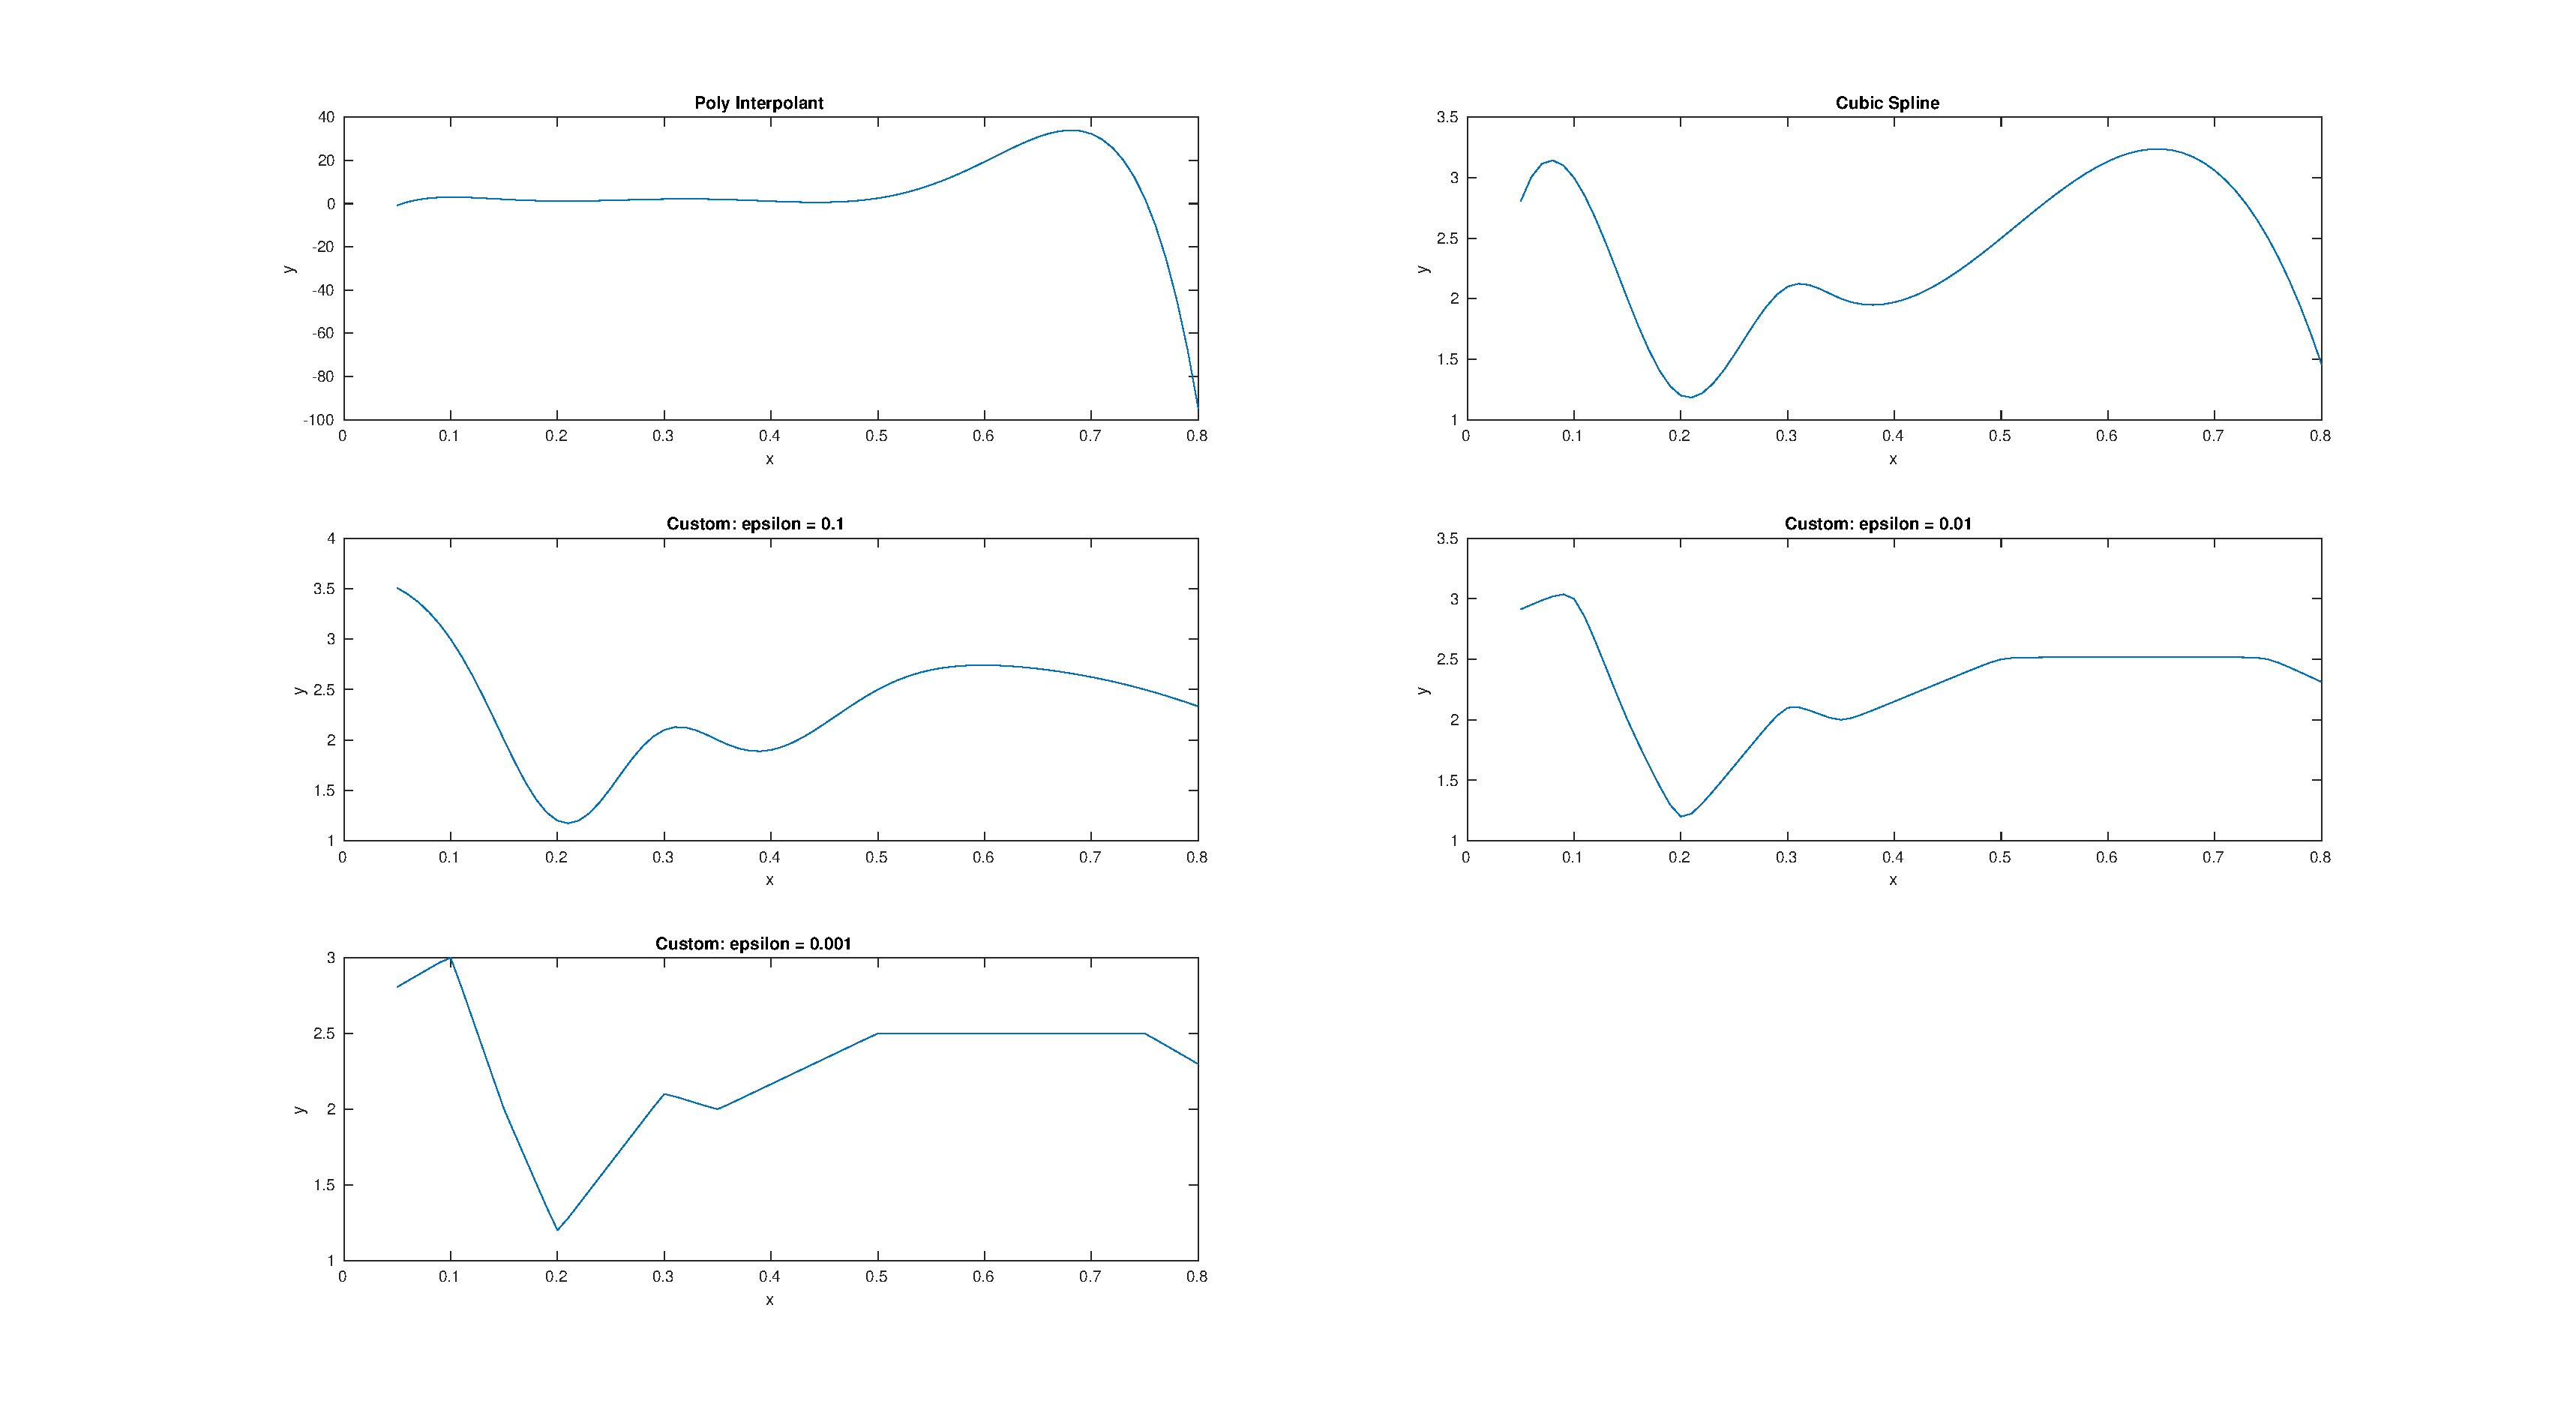
\includegraphics[width=15cm, height=15cm]{fig10}
  \caption{Matlab plots for different interpolant types}
  \end{figure}

  The figure shows the plots for the polynomial interpolant, cubic spline and the custom-interpolant method with $\epsilon =0.1,0.01, 0.001 and 0$. The matlab code is available as $Prob10.m$. The polynomial interpolant is of degree 6. Although it fits the data correctly, one of its bad property is due to its high degree and global control over all points, around the absiccae points where the data is not available for fitting, like from 0.5 to 0.7, the polynomial has the tendency to oscillate and explode to high values. In comparison, the cubic spline is significantly smooth and the curve is modeled closely to the given interpolating points.Since, the control here is local to set of 4 points, the degree is cubic. For the custom interpolants with the provided basis functions and tunable $\epsilon$, we see that as $\epsilon reduces$, the smoothness of the curve also reduces and around $\epsilon=0$, it becomes piecewise linear. 











\end{document}
